\documentclass[pdflatex,11pt]{aghdpl}
% \documentclass{aghdpl}               % przy kompilacji programem latex
% \documentclass[pdflatex,en]{aghdpl}  % praca w języku angielskim
\usepackage[polish]{babel}
\usepackage[utf8]{inputenc}

% dodatkowe pakiety
\usepackage{enumerate}
\usepackage{listings}
\lstloadlanguages{TeX}

%---------------------------------------------------------------------------

\author{Tomasz Drzewiecki, Joanna Gajda}
\shortauthor{T. Drzewiecki, J. Gajda}

\titlePL{Biometryczny System Kontroli Dostępu}
\titleEN{Biometric Access Control System}

\shorttitlePL{Biometryczny System Kontroli Dostępu} % skrócona wersja tytułu jeśli jest bardzo długi
\shorttitleEN{Biometric Access Control System}

\thesistypePL{Praca dyplomowa inżynierska}
\thesistypeEN{Bachelor's Thesis}

\supervisorPL{dr hab. inż. Marek Gorgoń}
\supervisorEN{Marek Gorgoń, Ph.D}

\date{2011}

\departmentPL{Katedra Automatyki}
\departmentEN{Department of Automatics}

\facultyPL{Wydział Elektrotechniki, Automatyki, Informatyki i Elektroniki}
\facultyEN{Faculty of Electrical Engineering, Automatics, Computer Science and Electronics}

\acknowledgements{Serdecznie dziękuję \dots tu ciąg dalszych podziękowań np. dla promotora, żony, sąsiada itp.}



\setlength{\cftsecnumwidth}{10mm}

%---------------------------------------------------------------------------

\begin{document}

\titlepages

\tableofcontents
\clearpage

\chapter{Wprowadzenie}
\label{cha:wprowadzenie}

%---------------------------------------------------------------------------

\section{Biometria oraz jej zastosowania ~w historii ~i współcześnie}
\label{sec:biometria}

Biometria jest, zgodnie ~z definicjami zaczerpniętymi ~z \cite{Ko75} oraz \cite{Bio01}, nauką obejmującą swoim zakresem badanie zmienności populacji organizmów. Wyniki tych badań, po opracowaniu ~z uwzględnieniem szerokiego zakresu metod statystyki matematycznej, wykorzystywane są ~w wielu różnych dziedzinach, między innymi antropologii, medycynie czy kryminalistyce. ~Z punktu widzenia techniki, zadaniem biometrii jest dokonywanie pomiarów istot żywych, ~w tym ~w szczególności cech charakterystycznych ludzi, które pozwoliłoby na automatyczne rozpoznawanie ~i weryfikację osób \cite{Bio01}\cite{Jain00}.

Identyfikacja biometryczna uwzględnia ~w swoich metodach dwa rodzaje cech człowieka ~\cite{Bio01}\cite{Bio02}\cite{Jain00}\cite{Jain08}:
\begin{itemize} 
\item fizyczne - na przykład tęczówka lub siatkówka oka, linie papilarne palców dłoni, układ naczyń krwionośnych, kształt dłoni, kształt ucha, obraz twarzy oraz rozkład temperatur na niej, charakterystyka uzębienia, DNA, 
\item behawioralne - sposób poruszania się, dynamika podpisu, sposób pisania na klawiaturze komputera czy cechy charakterystyczne głosu.
\end{itemize}

Wśród tradycyjnych metod identyfikacji bądź weryfikacji tożsamości możemy wyróżnić \cite{Jain00}\cite{Jain08}:
\begin{itemize}
\item oparte na posiadanych tokenach (ang. token-based), takich jak dowód tożsamości, paszport czy karta kredytowa,
\item oparte na posiadanej wiedzy (and. knowledge-based), czyli haśle, numerze PIN czy innym kodzie dostępu,
\end{itemize}
~W porównaniu ~z tradycyjnymi sposobami rozpoznawania i weryfikacji tożsamości, metody biometryczne okazują się być ~o wiele skuteczniejszym rozwiązaniem. Jest to spowodowane dużym prawdopodobieństwem zawodności tradycyjnych metod w sytuacjach, gdy posiadany token zostanie zgubiony, ulegnie kradzieży bądź sfałszowaniu lub kod dostępu unikalny dla danego użytkownika zostaje przechwycony albo zapomniany. Tradycyjne sposoby identyfikacji ~i weryfikacji nie gwarantują rozróżnienia pomiędzy właściwym posiadaczem danego tokenu lub wiedzy, ~a osobą, która weszła ~w posiadanie danych dostępowych ~w sposób bezprawny. Metody biometryczne wychodzą naprzeciw temu wymaganiu ze względu na tworzenie wzorca charakteryzującego człowieka w oparciu ~o informacje niesione przez unikalne dla niego cechy \cite{Jain00}. Ponadto, zwalniają one użytkownika ~z obowiązku tworzenia, zapamiętywania ~i przechowywania wiedzy lub przedmiotów koniecznych do identyfikacji/weryfikacji tożsamości \cite{Jain08}.  

Biometria miała zastosowanie już ~w przeszłości, na przykład poprzez pobieranie odcisków palców ~w celu potwierdzenia transakcji handlowych ~w czasach starożytnych, czy ~w trakcie rejestracji więźniów ~w XIX wieku \cite{Bio02}\cite{HF1}. Współcześnie, jest to jedna ~z najprężniej rozwijających się dziedzin bio- oraz teleinformatyki, której rozwiązania służą najczęściej jako forma kontroli dostępu ~i autoryzacji tożsamości użytkowników określonych pomieszczeń, urządzeń, danych ~i programów. Biometryczna identyfikacja tożsamości jest używana jako alternatywna, szybka ~i efektywna forma odprawy paszportowej pasażerów na lotniskach ~i granicach państwowych (poprzez analizowanie obszaru twarzy lub tęczówki oka) oraz do wyszukiwania osób ~w bazie ~i monitoringu czasu pracy ~w firmach \cite{Bio01}\cite{Bio02}.

Metody identyfikacji biometrycznej różnią się, poza formą analizy oraz wariantem analizowanych cech, skutecznością poprawności rozpoznawania danej osoby na podstawie próbek danych opisujących jej cechy, wymaganym stopniem zaangażowania analizowanej osoby ~w proces zbioru danych koniecznych do dokonania pomiarów oraz odpornością na oszustwa. Porównanie kilku metod biometrycznych zostało omówione ~w \cite{Gl11}. ~Z uwagi na dużą skuteczność ~i względnie prostą mierzalność, ~w niniejszej pracy skupiono się na identyfikacji w oparciu ~o obraz tęczówki oka.


%---------------------------------------------------------------------------

\section{Charakterystyka identyfikacji biometrycznej na podstawie tęczówki oka}
\label{sec:zawartoscPracy}

%~w rodziale~\ref{cha:pierwszyDokument} przedstawiono podstawowe informacje dotyczące struktury dokumentów ~w \LaTeX ~u. Alvis~\cite{Alvis2011} jest językiem 

Tęczówka ludzkiego oka jest jednym ~z najbardziej charakterystycznych elementów twarzy człowieka, indywidualnym ~i niepowtarzalnym ze względu na połączenie uwarunkowanego genetycznie koloru oraz złożonej struktury, wynikającej ~z różnorodnych procesów fizycznych ~i chemicznych, kształtujących ją ~w pierwszych latach ludzkiego życia [2][3]. Cechy te są wykorzystywane ~w procesie biometrycznej identyfikacji jednostki, który opiera się na zastosowaniu różnorodnych matematycznych metod rozpoznawania wzorców ~w algorytmach operujących na pobranym ~z użyciem specjalistycznej kamery obrazie oka.

Pobranie stabilnego ~i wolnego od zakłóceń obrazu ludzkiego oka wymaga pewnego stopnia współpracy ze strony osoby badanej, jednakże współczesne kamery ~i sprzęt projektowane specjalnie do tego typu identyfikacji, są  coraz lepiej przystosowane do automatycznej akwizycji obrazu wysokiej rozdzielczości. ~W związku ~z tym możliwe jest, iż ~z upływem czasu będą one mogły operować bez bezpośredniej kooperacji ze strony badanego.

Współcześnie stosowane kamery, wykorzystywane ~w celu akwizycji obrazu oka, operują we współpracy ~z czujnikami działającymi w środowisku bliskiej podczerwieni (NIR, ang. Near-Infra Red) lub obserwowalnej długości fali (VW, ang. Visible Wavelength). Promieniowanie podczerwone efektywnie wspomaga pobieranie tego typu obrazów ze względu na kilka czynników:
\begin{itemize} 
\item ~w zakresie widma NIR wyraźnie uwidaczniają się cechy posiadanej przez znaczną część populacji ludzkiej tęczówki ~w  odcieniach brązu,
\item promieniowanie to pomaga ~w likwidowaniu powstałych na powierzchni oka odblasków światła ~z otoczenia,
\item jest ono nieinwazyjne, w związku ~z czym nieszkodliwe dla oka.
\end{itemize}
Natomiast technika Visible Wavelength zachowuje informację na temat barwników przeważających w budowie tęczówki, co umożliwia pozyskanie danych dotyczących charakterystycznych wzorców występujących na obrazie. Obie technologie mają swoje zalety ~i wady; ich porównanie oraz próby połączenia ~w celu uzyskania dokładniejszego sposobu pozyskiwania zdjęć tęczówki ~i większej ilości niesionych wraz ~z tym informacji zostały opisane ~w pracy \cite{Hos10}. 

Proces identyfikacji na podstawie tęczówki, po uzyskaniu poprawnego obrazu przy pomocy kamery, dzieli się na kilka głównych etapów: \begin{itemize}
\item segmentacja, mająca na celu wyodrębnienie wewnętrznej ~i zewnętrznej granicy tęczówki na obrazie oka, wraz ~z szeregiem operacji, mających za zadanie wyeliminowanie zakłóceń na zdjęciu, ~w postaci otaczających tęczówkę rzęs, powiek czy powstałych ~w wyniku wpływu oświetlenia odblasków,
\item normalizacja, służąca do kompensacji deformacji tęczówki ~w związku ~z jej ewentualnym zwężeniem lub rozszerzeniem,
\item ekstrakcja cech tęczówki ~w celu uzyskania unikalnego kodu, podlegającego późniejszej analizie ~z zastosowaniem różnorodnych kryteriów, decydujących ~o identyfikacji bądź pozytywnym lub negatywnym wyniku weryfikacji tożsamości danej osoby.
\end{itemize}

Schemat przedstawiający działanie typowego systemu identyfikacji biometrycznej na podstawie tęczówki oka znajduje się na diagramie ~\ref{fig:identyfikacja}. Został on utworzony w oparciu ~o ogólne schematy działania typowych systemów identyfikacji biometrycznej, umieszczonych w ~\cite{Bio02} ~i \cite{Jain00}.
\begin{figure}[b]
\begin{center}
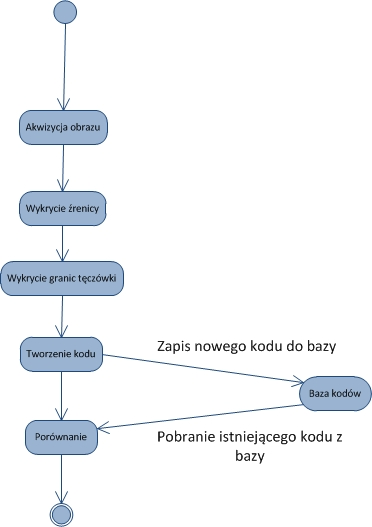
\includegraphics{schemat.jpg}
\caption{Schemat typowego systemu identyfikacji biometrycznej na podstawie tęczówki oka}
\label{fig:identyfikacja}
\end{center}
\end{figure}

Różnorodność metod segmentacji obszaru tęczówki oraz ekstrakcji cech ~i porównywania kodów została opisana ~w dalszych częściach pracy. Nie pokrywa ona oczywiście wszystkich metod obecnie znanych ~w tej dziedzinie, jednakże ~w niniejszej pracy starano się scharakteryzować jak największy ich podzbiór ~w oparciu ~o dostępną literaturę.


\section{Metody segmentacji obszaru tęczówki oka}
\label{sec:segmentacja}

Istnieje wiele metod segmentacji tęczówki \cite{PrAl06}. Pierwszą efektywnie zrealizowaną ~w systemie biometrycznym metodę zaproponował John Daugman \cite{Daugman}. Rozwiązanie to, jak wiele innych, późniejszych, opiera się na założeniu, że źrenica oraz tęczówka stanowią okręgi. Stosuje się ~w nim operator \ref{eq:daugman}.
\begin{equation}
\label{eq:daugman}
max_{r,x_{0},y_{0}}\left| G_{\sigma}(r) \frac{\delta}{\delta r}\int_{r,x_{0},y_{0}} \frac{~i(x,y)}{2\pi r}ds \right|
\end{equation}
gdzie:\\
$ x,y $ - położenie piksela na obrazie, \\
$ x_{0}, y_{0} $ - położenie środka okręgu na obrazie, \\
$ r $ - promień okręgu, \\
$ ~I(x,y) $ - jasność piksela na obrazie,\\
$ G_{\sigma}(r) $ - rozkład Gaussa.

Dzięki temu można odnaleźć środek okręgu oraz jego promień, dla których będziemy mieli największą wartość pochodnej względem najbliższego otoczenia. Ta metoda jest skuteczna dla obrazów, gdzie wyraźna jest granica między źrenicą ~a tęczówką oraz między tęczówką ~a rogówką. Częste jest ~w niej zastosowanie łuku dla szukania granicy między tęczówką ~a rogówką, ponieważ zdarza się, że część tęczówki jest zakryta przez powieki. [9]. Po skutecznie zrealizowanym algorytmie otrzymuje obraz podobny do przedstawionego na rysunku \ref{fig:przykladDaugman}.
\begin{figure}
\begin{center}
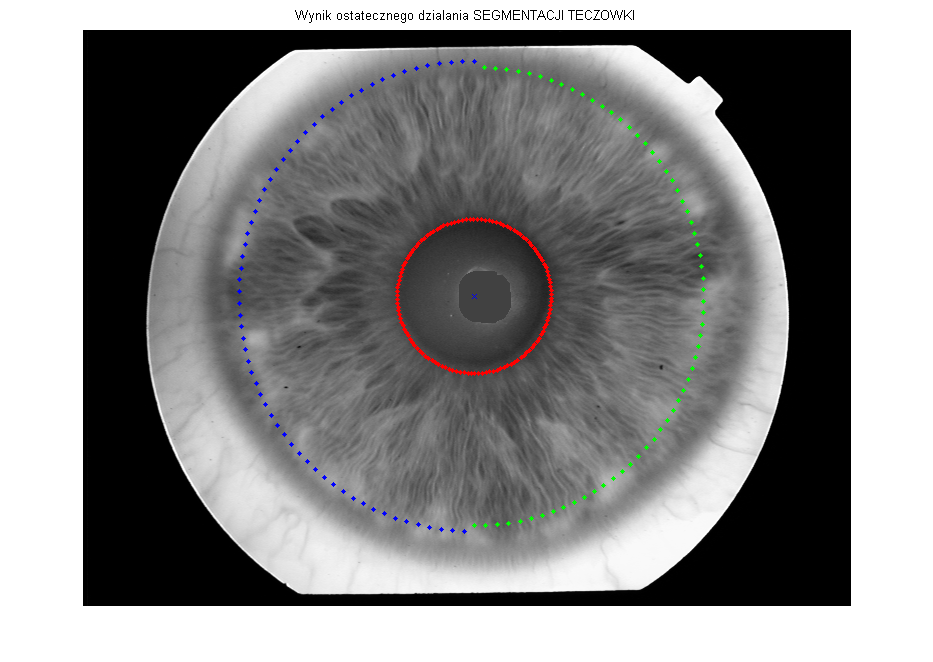
\includegraphics[scale=0.5]{calosc.png}
\caption{Obraz po realizacji algorytmu Daugmana}
\label{fig:przykladDaugman}
\end{center}
\end{figure}

Następnym rozwiązaniem jest metoda Wildes'~a \cite{Wildes}, która jest odmienna od patentu Daugmana. Algorytm ten jest realizowany ~w dwóch krokach. Pierwszym jest zamiana oryginalnego obrazu na obraz binarny ~z wyznaczonymi krawędziami, które są obecne na obrazie źródłowym. Najczęściej obraz pośredni jest tworzony za pomocą algorytmu Canny'ego. Na zmodyfikowanym obrazie stosowana jest transformacja Hough'~a [9], dzięki której można znaleźć środek okręgu opisującego tęczówkę oraz jego promień. Wadą tej metody jest trudność ustalenia progu binaryzacji.

Kolejnym sposobem segmentacji tęczówki jest rozwiązanie Camus'~a ~i Wildes'~a \cite{Camus}. Jest to metoda podobna do algorytmu Daugmana, która również polega na wyszukiwaniu tęczówki za pomocą maksymalizacji funkcji. ~W tym przypadku funkcją, którą maksymalizujemy jest równanie \ref{eq:camus_wildes} 
\begin{equation}
\label{eq:camus_wildes}
C=\sum_{\theta =1}^{n} ((n-1)\left|\left| g_{\theta,r} \right|\right| - \sum_{\varphi=\theta + 1 } ^{n} \left| \left| g_{\theta,r} - g_{\varphi,r} \right| \right| - \frac{I_{\theta,r}}{n}  )
\end{equation}
gdzie:\\
$ n $ - liczba dyskretnych wartości zmiennej biegunowej $ \theta $, \\
$ g_{\theta, r} $ - pochodna kierunkowa jasności obrazu.

Algorytm ten jest skuteczny głównie ~w przypadku, gdzie granica między tęczówką oraz rogówką oraz między tęczówką ~a źrenicą jest wyraźna oraz nie ma odblasków lub szumu.

\section{Metody generacji kodu tęczówki}
\label{sec:metodyGeneracjiKodu}

Istnieje wiele metod generacji kodu tęczówki. W patencie Daugmana zastosowano filtrację za pomocą filtrów Gabora \cite{Daugman}, których definicja we współrzędnych biegunowych jest przedstawiona w równaniu \ref{eq:gabor}.
\begin{equation}
\label{eq:gabor}
G(r,\theta) = e^{-2\pi i\omega (\theta - \theta 0)_{e}-(r - r0)2/a2_{e}-(\theta-\theta 0 )2/\beta 2}
\end{equation}
gdzie:\\
$r$ - promień we współrzędnych biegunowych, \\
$\theta$ - kąt w radianach we współrzędnych biegunowych, \\
$ \omega $ - częstotliwość, \\
$ \alpha, \beta $ - stałe.


Wybierane są punkty na obszarze tęczówki, w sposób pozwalający na poprawną analizę w przypadku zmiany jej rozmiaru. Jest to istotna kwestia, ponieważ w zależności od jasności otoczenia zmienia sie rozmiar źrenicy, co implikuję zmianę rozmiaru tęczówki. Punkty są następnie filtrowane ~z użyciem filtrów Gabora, dla różnych kierunków. W rezultacie otrzymywana jest (dla jednego punktu) liczba zespolona. Następuje kodowanie otrzymanej liczby w następujący sposób: 1, jeśli dana część jest większa od zera lub 0, jeśli jest mniejsza bądź równa zeru. W ten sposób otrzymywany jest bitowy kod (zwykle ~o długości 2048 bitów, jest to zależne od liczby wybranych punktów). Przykładowy wybór punktów jest przedstawiony na rysunku \ref{fig:przykladPunkty}

\begin{figure}
\begin{center}
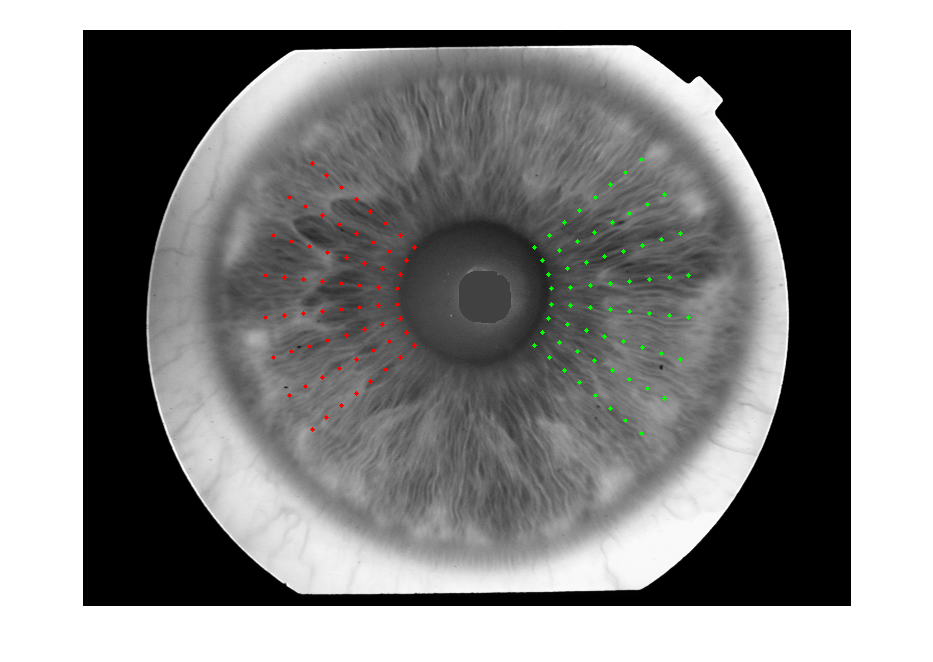
\includegraphics[scale=0.5]{punkty.png}
\caption{Przykładowy wybór punktów}
\label{fig:przykladPunkty}
\end{center}
\end{figure}

Inne podejście stosują Sun ~i Tan w swojej pracy \cite{TaSu09}. Proponują użycie tak zwanych ordinal measures do rozpoznawania na podstawie tęczówki. Wybiera się w nich dwa obszary, oblicza sumę jasności pikseli w tych obszarach ~i w zależności od tego, który obszar ma wyższą sumę, koduje się 1 lub 0. Ta metoda jest szybka oraz według twórców wykazuje dobre wyniki.

\section{Metody porównania kodów tęczówek}
\label{sec:metodyPorownaniaKodow}
Główną metodą stosowaną do porównywania kodów tęczówek jest, zaproponowane przez Daugmana, wyznaczanie odległości Hamminga. Odległość Hamminga określa liczbę bitów, których wartości są różne w dwóch porównywanych kodach. Zaletą tej metody jest szybkość obliczeń oraz prostota implementacji, dlatego została użyta w niniejszej pracy. Inne metody są przedstawione w pracy \cite{Gl11}.

\chapter{Realizacja biometrycznego systemu kontroli dostępu}
\label{cha:realizacja}
~W tym rozdziale przedstawiono sposób realizacji biometrycznego systemu do kontroli dostępu, wykorzystującego obraz tęczówki oka jako elementu na podstawie którego następuje rozpoznanie. System ten składa się ze stanowiska służącego do akwizycji obrazu oka, algorytmów przetwarzających pobrany obraz, generujących ~i porównujących kody tęczówek oraz aplikacji, mającej na celu ułatwienie korzystania ~z funkcji systemu ~i zapewniającej dostęp do bazy danych przechowującej informacje. Jest on rozbudowaną wersją systemu opracowanego ~w pracy \cite{Gl11}, opartą ~o zaprezentowaną ~w niej aplikację. ~W niniejszej pracy do poprzedniego systemu wprowadzony został szereg ulepszeń, zarówno pod kątem poprawy algorytmu działania, jak ~i wzbogacenia interfejsu użytkownika oraz bazy danych, służącej do przechowywania informacji dotyczących rozpoznawanych osób.
%~W tym rozdziale przedstawiono sposób realizacji systemu do kontroli dostępu wykorzystującego obraz tęczówki oka jako elementu na podstawie, którego następuje rozpoznanie. System składa się ze stanowiska do akwizycji obrazu tęczówki oka oraz aplikacji generującej kod tęczówki oraz porównującej kody ze sobą. Aplikacja składa się ~z kliku modułów: wykrycie źrenicy, wykrycie granic tęczówki, tworzenie kodu tęczówki oraz ewentualnie porównania wygenerowane kodu ~z już istniejącym.

\section{Stanowisko do akwizycji obrazu oka}
\label{sec:stanowisko}
Skonstruowane na potrzeby pracy stanowisko do akwizycji obrazu oka zostało oparte na pierwowzorze przedstawionym ~w pracy \cite{Gl11}. Rekonstrukcja nastąpiła ~w dwóch etapach. ~W pierwszym zastosowano kamerę ~o odmiennych od opisanych ~w pracy \cite{Gl11} parametrach, jednakże ~w związku ~z niewystarczającą jakością pobranych ~z jej pomocą obrazów, postanowiono podjąć kolejną próbę konstrukcji stanowiska, ~z użyciem poprzedniej kamery oraz obiektywu ~o lepszych parametrach.

Stanowisko złożone zostało ~z następujących elementów:
\begin{itemize}
 \item kamery cyfrowej, mającej za zadanie pobieranie obrazu ~w formie filmu bądź pojedynczych zdjęć,
 \item obiektywu ~o odpowiedniej ostrości ~i innych kluczowych parametrach,
 \item statywu, służącego do podtrzymywania ~i stabilizacji kamery,
 \item specjalnego stojaka, umożliwiającego poprawne ~i wygodne ułożenie głowy osoby, która jest identyfikowana,
 \item kartonowego pudła, ~w którym umieszczone zostały kamera ~i obiektyw oraz do którego częściowo wsunięty został stojak,
 \item lampy, generującej oświetlenie ~w celu uzyskania jak najwęższego rozmiaru źrenicy oka ~z przytwierdzonym fragmentem tworzywa pleksi rozpraszającego promienie światła.
 \end{itemize}

Podczas pierwszej próby konstrukcji stanowiska, jako urządzenie pobierające obraz oka wybrano kamerę firmy , ~o następujących parametrach:

Wybór urządzenia był ograniczony zasobami laboratorium, ~w którym było tworzone stanowisko. Kamera została umieszczona na statywie, ~w celu regulacji jej położenia ~i stabilizacji pobieranego obrazu.

Do wybranej kamery należało dobrać obiektyw. Ponieważ podstawowym celem akwizycji było otrzymanie ostrego obrazu ~o dużym powiększeniu oraz odpowiedniej głębi ostrości, należało wybrać obiektyw ~o możliwie dużej ogniskowej. Zdecydowano się wykorzystać najlepszy dostępny ~w laboratorium obiektyw, !!!!!TU WSTAWIĆ NAZWĘ!!!!.

Po odpowiednim ustawieniu opisanych urządzeń, na wprost kamery umieszczono stojak, mający na celu podtrzymanie głowy osoby identyfikowanej. Został on ustawiony na wysokości odpowiadającej położeniu komfortowemu dla większości osób, ~z umożliwieniem jego ewentualnej modyfikacji.

Następnie podjęto próby akwizycji obrazu. Po zapisaniu zdjęć pobranych przy pomocy kamery, istotnym problemem okazały się być odblaski, powstałe na powierzchni oka ~w wyniku odbicia światła zewnętrznego, pochodzącego ~z otoczenia lub sztucznych źródeł, takich, jak żarówki. Odblaskami stanowiącymi największą przeszkodę były obecne na tęczówce oraz źrenicy, ponieważ te elementy obrazu są kluczowe dla dalszej analizy. Najprostszym sposobem eliminacji tego rodzaju zakłóceń jest ograniczenie dostępu promieni świetlnych ~z otoczenia do obszaru, ~w którym pobierany jest obraz. Udało się to zrealizować, podobnie jak ~w \cite{Gl11}, za pomocą umieszczenia kamery ~w kartonowym pudełku, na granicy którego ustawiono stojak stabilizujący głowę. Metoda ta pozwoliła na ograniczenie odblasków do minimum oraz uzyskanie odpowiedniej ostrości obrazu poprzez unieruchomienie głowy osoby identyfikowanej.

Wadą zastosowanego rozwiązania było jednak zmniejszenie jasności uzyskiwanych obrazów. Przyczyniło się to do rozszerzenia źrenicy oka, co miało negatywny wpływ na długość promienia tęczówki. ~W celu rozjaśnienia obrazu użyto więc oświetlacza IR oraz lampy umieszczonej na kamerze, której zadaniem było oświetlenie oka badanej osoby ~i ~w konsekwencji zwężenie obszaru źrenicy. Takiego rodzaju oświetlenie również tworzy odblaski, lecz ~w tym wypadku mogą być one wykorzystane przez algorytm wykrywający źrenicę. Jest to możliwe, ponieważ ~z uwagi na umiejscowienie lampy odblask powstaje na środku źrenicy, dzięki czemu ułatwiona zostaje jej lokalizacja. (Dodać coś ~o oświetlaczu IR). Obraz jest zapisywany ~w skali szarości.

Pobierany obraz zapisywany był ~w skali szarości ~i formacie BMP, co umożliwiło łatwiejsze jego przetwarzanie przez algorytm. Po wykonaniu odpowiedniej ilości testów programu na pobranych zdjęciach, okazało się jednak, iż nie cechowały się one wystarczająco wysoką jakością, która konieczna była dla poprawnego działania algorytmów generujących ~i porównujących kody tęczówek. ~W związku ~z tym, niezbędna była ponowna rekonstrukcja stanowiska, tym razem ~z zastosowaniem kamery ~o sprawdzonej skuteczności pobierania obrazu, użytej ~w pracy \cite{Gl11}.

W trakcie drugiej próby konstrukcji stanowiska, zdecydowano się na zastosowanie urządzenia firmy ~o parametrach: . Problemem wywołującym trudności podczas pobierania obrazów przy pomocy poprzedniej kamery była jej mała rozdzielczość, co udało się pokonać stosując nową kamerę. Ponadto, wewnątrz kartonowego pudełka jasność otoczenia była zbyt niska, pomimo użytej lampy, jednak udało się to zniwelować wyłącznie ~z użyciem oświetlacza IR, dzięki czemu na obrazie widocznych było mniej odblasków. Oświetlacz został zamontowany na kamerze.

Postanowiono pozostać przy obiektywie, który został użyty podczas pierwszej konstrukcji stanowiska. Pozostałe części, takie, jak kartonowe pudełko, stojak, statyw oraz oświetlacz IR również nie uległy modyfikacji.

\section{Część biometryczna - wykrywanie tęczówki oka na obrazie ~i identyfikacja bądź weryfikacja tożsamości na jej podstawie}
\subsection{Wykrywanie źrenicy na pobranym obrazie}
\label{sec:wykrycieZrenicy}

Część algorytmu odpowiedzialna za wykrycie źrenicy ma za zadanie odnalezienie tej części oka ludzkiego na obrazie oraz opisanie jej kształtu ~w formie okręgu ~o odpowiednich parametrach. Zadanie to jest realizowane ~z wykorzystaniem opisanego ~w podrozdziale \ref{sec:stanowisko} odblasku, pochodzącego od lampy ustawionej na kamerze, Powinien on znajdować się ~w centrum źrenicy, dlatego też konieczne jest ustawienie we właściwej pozycji osoby, której zdjęcie jest pobierane przez kamerę. Odblask jest jednym ~z najjaśniejszych punktów na obrazie. ~W związku ~z tym, wykrycie odblasku odbywa się poprzez wykorzystanie binaryzacji ~z progiem 254. ~W wyniku tej operacji na obrazie zostają tylko piksele najjaśniejsze (jak na rysunku \ref{fig:binaryzacja}). Niestety na wielu ujęciach odblask na źrenicy nie jest jedynym, który jest widoczny na obrazie. Pozostałe mogą znajdować się ~w różnych miejscach: na białku oka lub na skórze. Można ten fakt wykorzystać poprzez analizę otoczenia znalezionych odblasków. 

\begin{figure}
\begin{center}
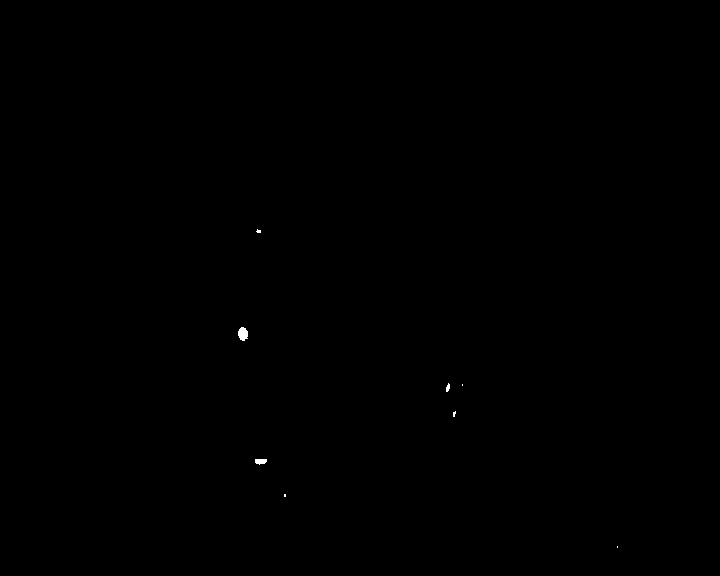
\includegraphics[scale=0.5]{binaryzacja.jpg}
\caption{Obraz po binaryzacji, jasne punkty to znalezione odblaski}
\label{fig:binaryzacja}
\end{center}
\end{figure}

Najistotniejszy dla dalszych etapów algorytmu odblask znajduje się ~w otoczeniu źrenicy, ~a więc jednego ~z najciemniejszych obszarów obrazu; otoczenie pozostałych odblasków jest ~o wiele jaśniejsze (skóra lub białko oka). ~W obrazie uzyskanym po binaryzacji wyszukiwane są piksele odblasku. ~W momencie znalezienia każdego kolejnego piksela odblasku analizowane jest jego otoczenie. Sprawdzanych jest po 10 punków na ukos ~w górę ~z lewej ~i prawej strony ~w odległości do 11 do 20 pikseli. Jeśli większość z nich ma jasność poniżej 60 to analizowany piksel jest uznawany za piksel odblasku znajdującego się na źrenicy. ~W takiej sytuacji wyszukiwanie zostaje zakończone i następuje dalsza cześć algorytmu.

Następnie wyszukiwany jest cały odblask. Odbywa się to poprzez analizę otoczenia (kwadratu o boku 50 pikseli oraz środku ~w miejscu już znalezionego fragmentu) znalezionego punktu. Sprawdzany jest każdy piksel ~w wybranym otoczeniu i uznawany jest za element odblasku ~w sytuacji, gdy jego jasność jest większa niż 240. Przykład wyniku przeprowadzonych operacji jest przedstawiony na rysunku \ref{fig:dobryOdblask}.

\begin{figure}
\begin{center}
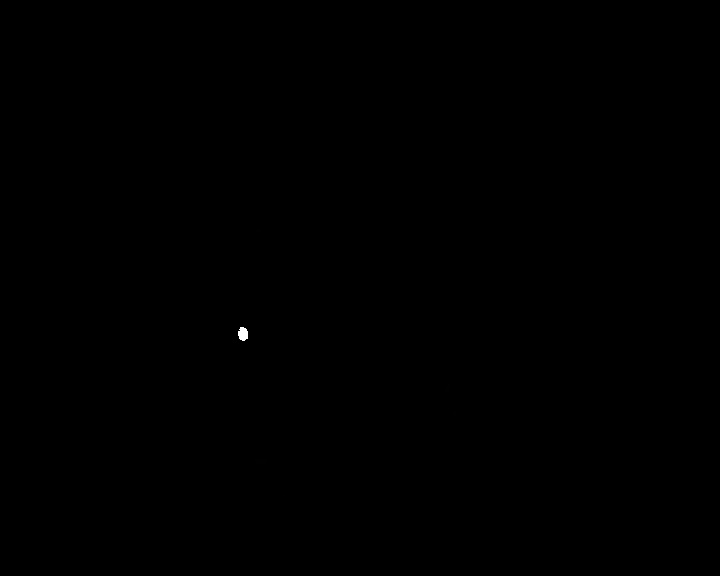
\includegraphics[scale=0.5]{odblask.jpg}
\caption{Obraz po realizacji algorytmu poszukiwania odblasku na źrenicy}
\label{fig:dobryOdblask}
\end{center}
\end{figure}

Po znalezieniu wszystkich pikseli należących do odblasku, jego kształt jest aproksymowany przy pomocy koła, którego środek jest przyjmowany jako środek źrenicy. Mając środek źrenicy można zastosować metodę ,,eksplodujących okręgów'', zaczerpniętych ~z patentu Daugmana.  Szukany jest największy wzrost jasności pikseli na rozszerzającym się okręgu (z uwagi na to, że źrenica jest ciemna, ~a tęczówka jest jaśniejsza). Znaleziony okrąg określa źrenicę. Niestety dla zarejestrowanych obrazów metoda nie okazała się skuteczna. Z tego powodu zastosowano nieco odmienną metodę. Wyszukiwanie odbywa się na promieniach, to znaczy wybierane są 72 promienie ~o różnych kierunkach ~i na każdym wyszukiwany jest największy wzrost jasności. Dla znalezionych punktów wyszukuje się najmniejszy okrąg, ~w którym zawierają się wszystkie punkty. Stosowany jest algorytm zaimplementowany ~w bibliotece OpenCV. Znaleziony okrąg określa źrenicę. Przykład obrazu ~z wykrytą źrenicą jest przedstawiony na rysunku \ref{fig:zrenicaNasza}.

\begin{figure}
\begin{center}
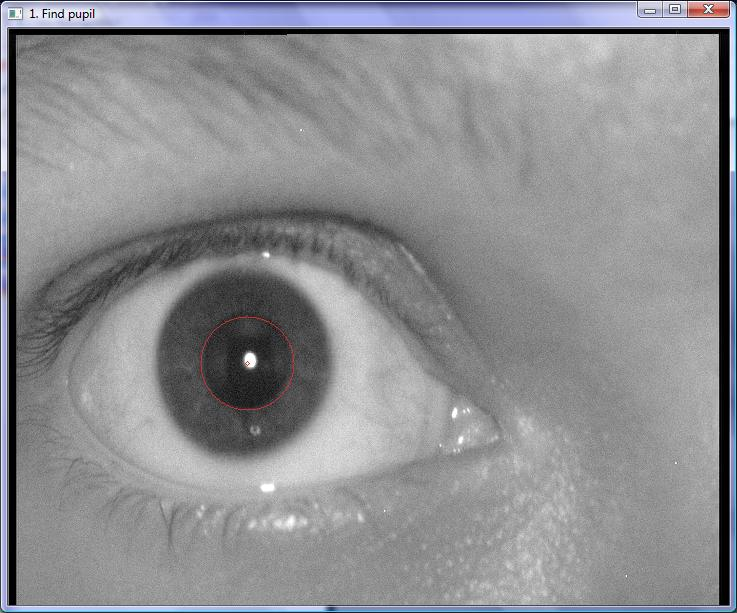
\includegraphics[scale=0.5]{zrenica.jpg}
\caption{Wykryta źrenica}
\label{fig:zrenicaNasza}
\end{center}
\end{figure}

Po zmianie kamery algorytm wykrywania źrenicy został zmieniony. Było to spowodowane poprawą jasności zdjęcia oraz zmianą położenia niektórych elementów stanowiska. Odblask na źrenicy, wcześniej będący się ~w środku źrenicy po zmienie stanowiska znajduje się ponad środkiem. ~W związku ~z tym nie można go wykorzystać do ustalenia środka źrenicy.

Można natomiast wykorzystać wykrycie odblasku do oszacowania, ~w którym miejscu na obrazie znajduje się źrenica. Pozwala to ograniczyć wielkość obrazu podlegającemu późniejszym przekształceniom. Wybierany jest kwadrat ~o boku 440 pikseli. Taki obszar jest wystarczający, ponieważ promień źrenicy na rejestrowanych obrazach nie przekracza 150 pikseli. Taki zabieg pozwala na osiągnięcie dwóch korzyści. Pierwszą jest zmniejszenie obszaru, który podlega przekształceniom co przyśpiesza działanie progami. Drugą jest ograniczenie innych obiektów na zdjęciu, jak brwi czy rzęsy, które mogą być uznane podczas binaryzacji za fragmenty źrenicy. Pozwala to na ograniczenie błędów podczas segmentacji. Przykładowy wybór obszaru jest przedstawiony na rysunku \ref{fig:obszar}.

\begin{figure}
\begin{center}
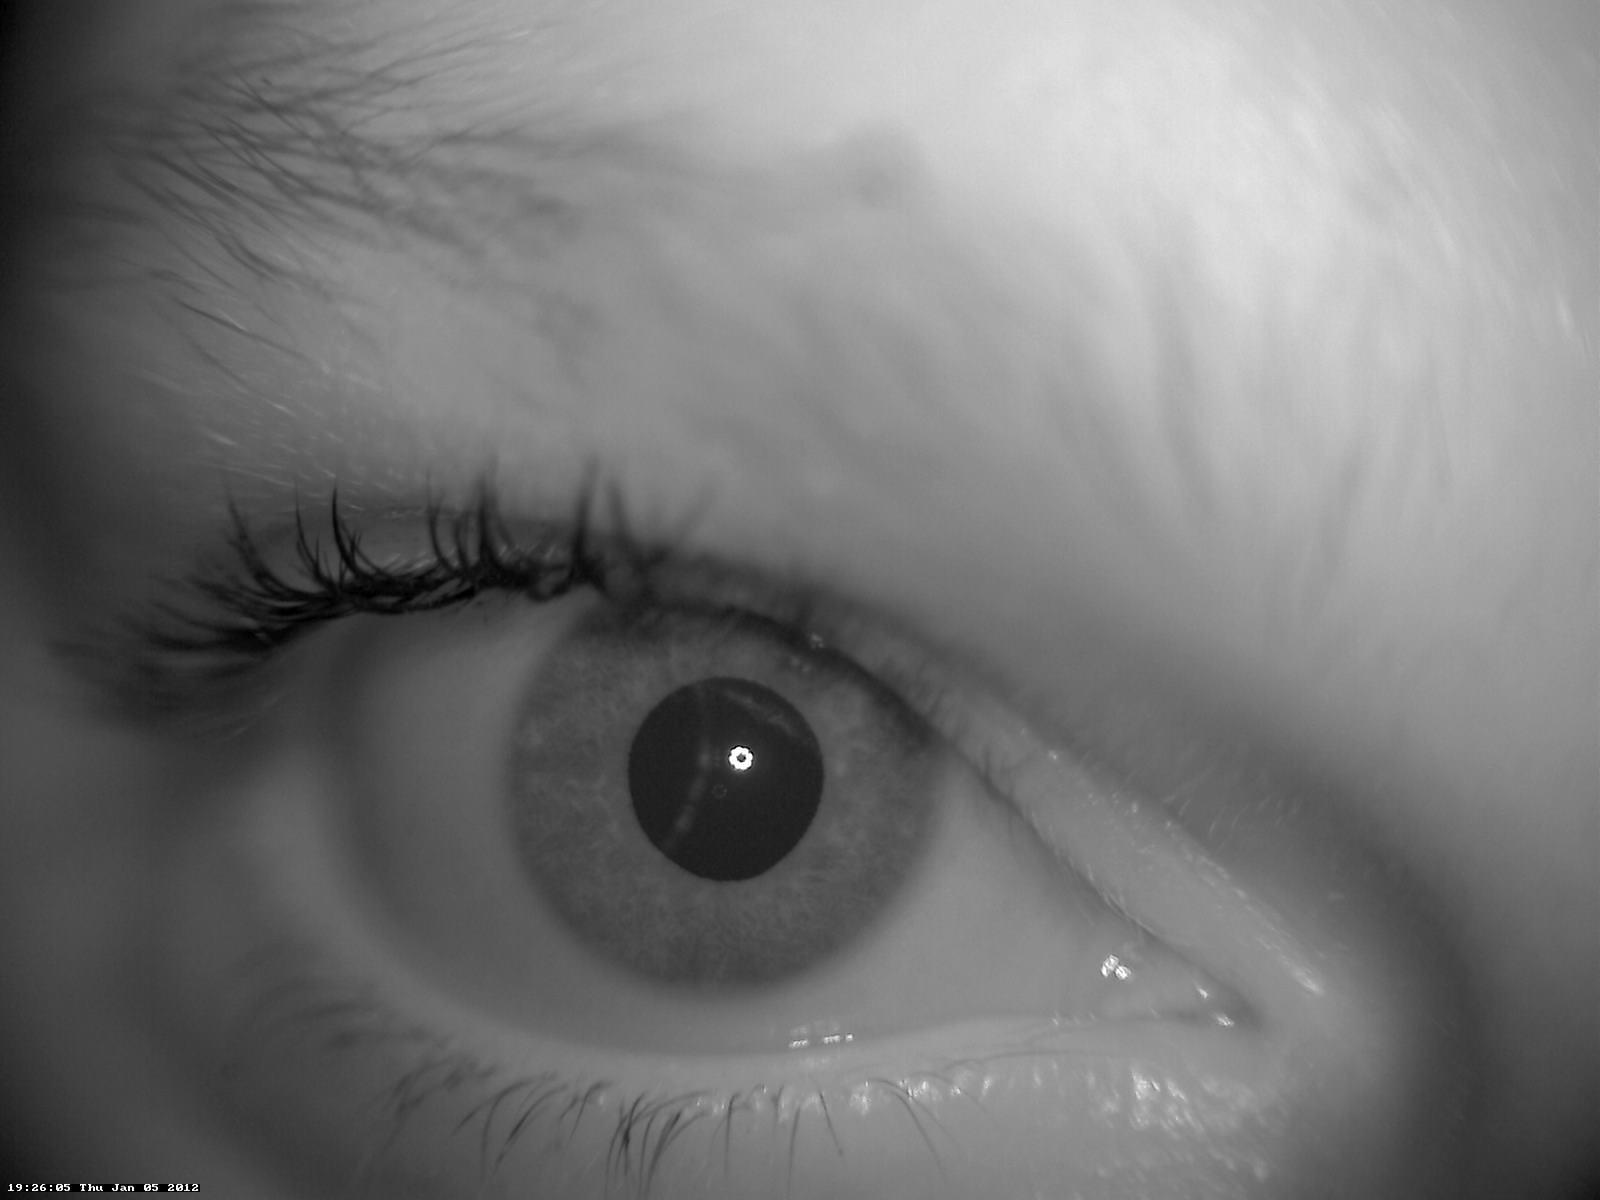
\includegraphics[scale=0.25]{obszar.jpg}
\caption{Obraz z zaznaczonym obszarem do dalszych przekształceń}
\label{fig:obszar}
\end{center}
\end{figure}

Wykrycie odblasku na źrenicy jest realizowane za pomocą algorytmu opisanego wcześniej ze zmianami. Analizowane są punkty ~w większej odległości od znalezionego piksela, ponieważ dla obrazów rejestrowanych za pomocą drugiej wybranej kamery obrazy mają większą rozdzielczość oraz sam odblask ma inny kształt oraz wielkość. Nie jest konieczne wyszukiwanie całego odblasku, ponieważ dowolny piksel odblasku będzie wystarczającym środkiem wybieranego fragmentu obrazu ~i różnica rzędu kilku pikseli nie ma znaczenia dla dalszych przekształceń.

~W opisanym obszarze przeprowadzane są następujące operacje:
\begin{itemize}
\item Najpierw stosowana jest binaryzacja ~z dwoma programi, wybierane są piksele należące do źrenicy (o jasności mniejszej niż 60) oraz piksele należące do odblasku (o jasności 255). Dzięki temu, otrzymuje bardziej zwarty obszar źrenicy. Po tej operacji powstaje obraz \ref{fig:binaryzacja2}, na którym widać większą część źrenicy.
\begin{figure}
\begin{center}
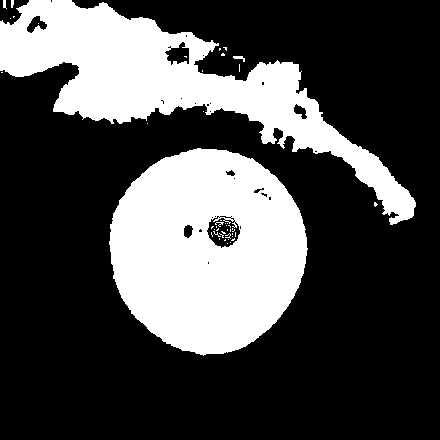
\includegraphics[scale=0.5]{binaryzacja2.jpg}
\caption{Obraz po binaryzacji}
\label{fig:binaryzacja2}
\end{center}
\end{figure}
\item Zamknięcie, po którym obszary znajdujące się ~w środku źrenicy ~w otoczeniu odblasku, które mają mniejszą jasność niż on sam zostają włączone do obszaru źrenicy. Na obrazie \ref{fig:zamkniecie2} po tej operacji wyraźnie widać, że źrenica jest wyznaczona ~w całości.
\begin{figure}
\begin{center}

\includegraphics[scale=0.5]{zamkniecie.jpg}
\caption{Obraz po operacji zamkniecia}
\label{fig:zamkniecie2}
\end{center}
\end{figure}
\item Dwuktrotne otwarcie, po którym usuwane są ~w większej części obszary rzęs, które pozostają po wcześniejszych operacjach. Czasem po binaryzacji powstaje obraz, na którym rzęsy są połączone ze źrenicą. Ta operacja pozwala rozdzielić je od siebie.
\begin{figure}
\begin{center}

\includegraphics[scale=0.5]{otwarcie2.jpg}
\caption{Obraz po operacjach otwarcia}
\label{fig:otwarcie2}
\end{center}
\end{figure}
\item Czyszczenie brzegów ~w ramach wybranego wcześniej obszaru. Po tej operacji na obrazie zostaje sama źrenica ~i znikają ewentualne pozostałości po wykrytych rzęsach. Jest to ostatni etap wyznaczania obszaru źrenicy ~i otrzymujemy obraz \ref{fig:zrenica2}.
\begin{figure}
\begin{center}

\includegraphics[scale=0.5]{roi2.jpg}
\caption{Obraz po wyczyszczeniu brzegów}
\label{fig:zrenica2}
\end{center}
\end{figure}
\end{itemize}


\section{Wykrycie tęczówki}
\label{sec:wykrycieTeczowki}
Algorytm odpowiedzialny za wykrycie tęczówki oparty został na użytym ~w pracy \cite{Gl11}. Przykładowy obraz ~z wykrytą tęczówką jest przedstawiony na rysunku \ref{fig:teczowkaNasza}.
\begin{figure}
\begin{center}
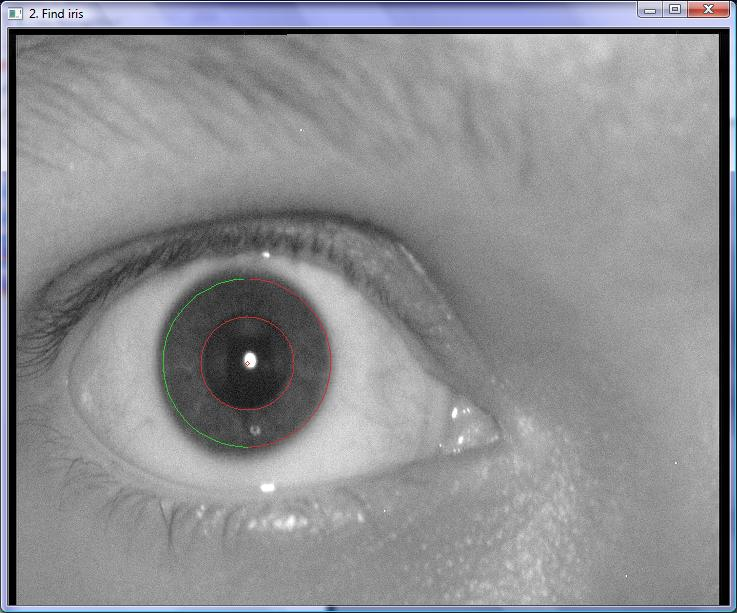
\includegraphics[scale=0.5]{teczowka.jpg}
\caption{Obraz po realizacji algorytmu poszukiwania granic tęczówki}
\label{fig:teczowkaNasza}
\end{center}
\end{figure}

\section{Ekstrakcja cech tęczówki}
\label{sec:ekstrakcja}
Zadaniem części algorytmu odpowiedzialnej za ektrakcję cech tęczówki jest ograniczenie ilości danych reprezentujących daną tęczówkę. Po przeprowadzeniu tej operacji zostaje utworzony wektor ~o długości 2048 bitów. Dzięki temu można znacznie zmniejszyć rozmiar przechowywanych danych, potrzebnych do poprawnego rozpoznania osoby. Ważne jest, by otrzymany wektor był wyraźnie odmienny dla różnych osób oraz aby dla jednej osoby różne zdjęcia generowały podobny zestaw bitów. 

~W celu określenia cech danej tęczówki stosuje się filtry Gabora określone wzorem \ref{eq:Gabor}:
\begin{equation}
\label{eq:Gabor}
g(x,y) = s(x,y)\cdot w_{r}(x,y)
\end{equation}
gdzie:\\
$s(x,y)$ - sinusoida zespolona określona wzorem \ref{eq:sin_complex},\\
$w_{r}(x,y)$ - ,,koperta Gaussowska'' określona wzorem \ref{eq:koperta_Gaussa}.\\
\begin{equation}
\label{eq:sin_complex}
s(x,y) = e^{i(2 \pi F_{0} \cdot (xcos(\omega_{0}) + ysin(\omega_{0})) + P)}
\end{equation}
gdzie:\\
$F_{0}$ - amplituda,\\
$\omega_{0}$ - kierunek filtru,\\
$P$ - przesunięcie filtru.\\
\begin{equation}
\label{eq:koperta_Gaussa}
w_{r}(x,y) = K \cdot e^{-\pi(a^{2}(x-x_{0})_{r}^{2}) + b^{2}(y-y_{0})_{r}^{2}}
\end{equation}
gdzie:\\
$K$ - amplituda koperty Gaussa,\\
$a$ - skalowanie koperty Gaussa w osi x,\\
$b$ - skalowanie koperty Gaussa w osi y,\\
$(x-x_{0})_{r}$ - jest określone równaniem \ref{eq:xr},\\
$(y-y_{0})_{r}$ - jest określone równaniem \ref{eq:yr}.\\
\begin{equation}
\label{eq:xr}
(x-x_{0})_{r} = (x-x_{0})cos(\theta)+(y-y_{0})sin(\theta)
\end{equation}
\begin{equation}
\label{eq:yr}
(y-y_{0})_{r} = (x-x_{0})sin(\theta)+(y-y_{0})cos(\theta)
\end{equation}
gdzie:\\
$x_{0}$ - położenie szczytu koperty Gaussa na osi x,\\
$y_{0}$ - położenie szczytu koperty Gaussa na osi y,\\
$\theta$ - obrót koperty Gaussa.

~W niniejszej pracy używane są filtry Gabora ~o wielkości 11 na 11 pikseli ~o następujących parametrach:\\
$F_{0} = \frac{8}{\pi}$,\\
$P = 0$,\\
$a = \frac{1}{2}$,\\
$b = \frac{3}{10}$,\\
$\theta = \pi / 4$,\\
$x_{0} = 0$, $y_{0} = 0$ - punkt $(0,0)$ znajduje się w środku filtru,\\
Używanych jest 8 kierunków $\omega_{0} =\frac {k \cdot \pi} {8} $ dla $k = 0, 1, ..., 8$.

Obraz jest przetwarzany ~z użyciem wspomnianych filtrów. Po tym zabiegu otrzymujemy współczynniki zespolone, które sumujemy ~w pewnych obszarach. Obszary wybierane są na powierzchni tęczówki ~w punktach zależnych od jej rozmiaru. Jest to spowodowane tym, że ~w zależności od jasności otoczenia źrenica zwiększa się lub zmniejsza, co powoduje zwężenie lub rozszerzenie tęczówki. Otrzymane sumy kodowane są ~w ten sposób, że osobno rozpatrując część rzeczywistą ~i urojoną, zapisywane jest 1 ~w przypadku, gdy suma jest większa od zera oraz 0 jeśli jest mniejsza lub równa. ~W ten sposób otrzymujemy 2 bity na jeden obszar. Ponieważ stosowane jest 8 różnych orientacji filtru Gabora, potrzebny jest wybór 2048/(2*8) = 128 obszarów. Obszary wybierane są po dwóch stronach tęczówki, więc wymagany jest wybór 64 obszarów na każdej stronie. Przykład wyznaczonych obszarów przedstawiony jest na rysunku \ref{fig:obszaryNasze}.

\begin{figure}
\begin{center}
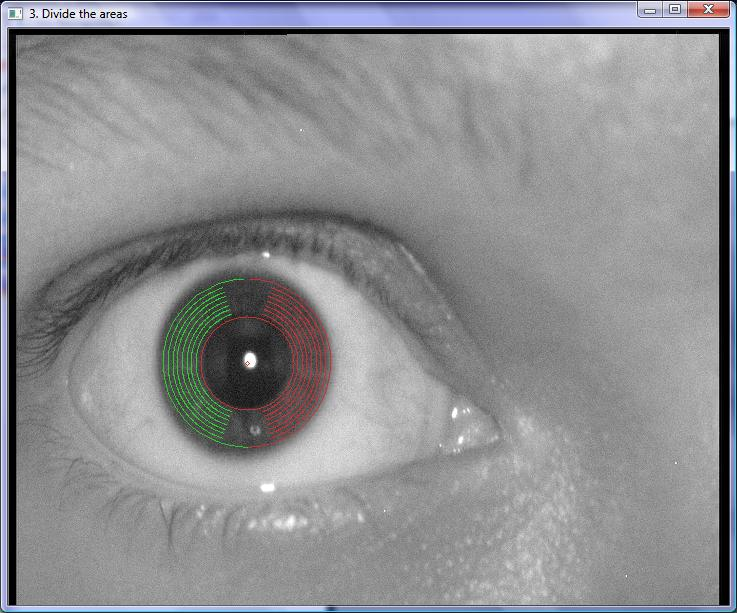
\includegraphics[scale=0.5]{obszary.jpg}
\caption{Obraz ~z zaznaczonymi obszarami używanymi do tworzenia kodu tęczówki}
\label{fig:obszaryNasze}
\end{center}
\end{figure}

\subsection{Porównanie kodów tęczówki}
\label{subsec:porownanieKodow}
~W celu określenia, czy dane dwie tęczówki należą do tej samej osoby, niezbędne jest porównanie otrzymanych kodów. Porównanie wykonywane jest za pomocą operacji XOR zgodnie ze wzorem \ref{eq:Hamming}.
\begin{equation}
\label{eq:Hamming}
H = \frac{\sum XOR(A,B)}{2048}
\end{equation}
gdzie:
$A, B$ - porównywane kody tęczówek, każdy ~o długości 2048 bitów.\\
Po tej operacji wartość $H$ określa procent różnych pikseli dla dwóch różnych kodów.

Głowa danej osoby może być ~w pozycji nieznacznie obróconej ~w trakcie pobierania zdjęcia służącego identyfikacji ~w stosunku do zdjęcia, ~na podstawie  którego powstał kod zapisany  ~w bazie. ~W celu zminimalizowania błędu stosowana jest rotacja jednego ~z porównywanych kodów. Kod jest przesuwany ~w obydwie strony ~o dwa piksele (ponieważ ~z jednej lokalizacji na obrazie otrzymujemy dwa bity kodu). Wykonywanych jest 9 porównań kodów. Wybierana jest najniższa wyliczona wartość odległości Hamminga. Ustalonym progiem zgodności dwóch kodów jest 0.18 \cite{Daugman}.


%\chapter{Pierwszy dokument}
\label{cha:pierwszyDokument}

W rozdziale tym przedstawiono podstawowe informacje dotyczące struktury prostych plików \LaTeX a. Omówiono również metody kompilacji plików z zastosowaniem programów \emph{latex} oraz \emph{pdflatex}.

%---------------------------------------------------------------------------

\section{Struktura dokumentu}
\label{sec:strukturaDokumentu}

Plik \LaTeX owy jest plikiem tekstowym, który oprócz tekstu zawiera polecenia formatujące ten tekst (analogicznie do języka HTML). Plik składa się z dwóch części:
\begin{enumerate}%[1)]
\item Preambuły -- określającej klasę dokumentu oraz zawierającej m.in. polecenia dołączającej dodatkowe pakiety;

\item Części głównej -- zawierającej zasadniczą treść dokumentu.
\end{enumerate}



\begin{lstlisting}
\documentclass[a4paper,12pt]{article}      % preambula
\usepackage[polish]{babel}
\usepackage[latin2]{inputenc}
\usepackage[T1]{fontenc}
\usepackage{times}

\begin{document}                           % część główna

\section{Sztuczne życie}

% treść

\end{document}
\end{lstlisting}

Nie ma żadnych przeciwskazań do tworzenia dokumentów w~\LaTeX u w~języku polskim. Plik źródłowy jest zwykłym plikiem tekstowym i~do jego przygotowania można użyć dowolnego edytora tekstów, a~polskie znaki wprowadzać używając prawego klawisza \texttt{Alt}. Jeżeli po kompilacji dokumentu polskie znaki nie są wyświetlane poprawnie, to na 95\% źle określono sposób kodowania znaków (należy zmienić opcje wykorzystywanych pakietów).


%---------------------------------------------------------------------------

\section{Kompilacja}
\label{sec:kompilacja}


Załóżmy, że przygotowany przez nas dokument zapisany jest w pliku \texttt{test.tex}. Kolejno wykonane poniższe polecenia (pod warunkiem, że w pierwszym przypadku nie wykryto błędów i kompilacja zakończyła się sukcesem) pozwalają uzyskać nasz dokument w formacie pdf:
\begin{lstlisting}
latex test.tex
dvips test.dvi -o test.ps
ps2pdf test.ps
\end{lstlisting}
%
lub za pomocą PDF\LaTeX:
\begin{lstlisting}
pdflatex test.tex
\end{lstlisting}

Przy pierwszej kompilacji po zmiane tekstu, dodaniu nowych etykiet itp., \LaTeX~tworzy sobie spis rozdziałów, obrazków, tabel itp., a dopiero przy następnej kompilacji korzysta z tych informacji.

W pierwszym przypadku rysunki powinny być przygotowane w~formacie eps, a~w~drugim w~formacie pdf. Ponadto, jeżeli używamy polecenia \texttt{pdflatex test.tex} można wstawiać grafikę bitową (np. w formacie jpg).



%---------------------------------------------------------------------------

\section{Narzędzia}
\label{sec:narzedzia}


Do przygotowania pliku źródłowego może zostać wykorzystany dowolny edytor tekstowy. Niektóre edytory, np. Emacs, mają wbudowane moduły ułatwiające składanie tekstów w LaTeXu (kolorowanie składni, skrypty kompilacji, itp.).

Jednym z bardziej znanych środowisk do składania dokumentów  \LaTeX a jest {\em Kile}. Aplikacja dostępna jest dla środowiska KDE począwszy od wersji 2. Zawiera edytor z podświetlaną składnią, zestawy poleceń \LaTeX a, zestawy symboli matematycznych, kreatory tabel, macierzy, skrypty kompilujące i konwertujące podpięte są do poleceń w menu aplikacji (i pasków narzędziowych), dostępne jest sprawdzanie pisowni, edytor obsługuje projekty (tzn. dokumenty składające się z~wielu plików), umożliwia przygotowanie i~zarządzanie bibliografią, itp.

Na stronie \underline{\texttt{http://kile.sourceforge.net/screenshots.php}} zamieszczono kilkanaście zrzutów ekranu środowiska {\em Kile}, które warto przejrzeć, by wstępnie zapoznać się z~możliwościami programu.

Bardzo dobrym środowiskiem jest również edytor gEdit z wtyczką obsługującą \LaTeX a. Jest to standardowy edytor środowiska Gnome. Po instalacji wtyczki obsługującej \LaTeX a, edytor nie ustępuje funkcjonalnościom środowisku Kile, a jest zdecydowanie szybszy w działaniu. Lista dostępnych wtyczek dla tego edytora znajduje się pod adresem \underline{\texttt{http://live.gnome.org/Gedit/Plugins}}. Inne polecane wtyczki to: 
\begin{itemize}
\item Edit shortcuts -- definiowanie własnych klawiszy skrótu;
\item Line Tools -- dodatkowe operacje na liniach tekstu;
\item Multi-edit -- możliwość jednoczesnej edycji w wielu miejscach tekstu;
\item Zoom -- zmiana wielkości czcionki edytora z użyciem rolki myszy;
\item Split View -- możliwość podziału okna edytora na 2 części. 
\end{itemize}



%---------------------------------------------------------------------------

\section{Przygotowanie dokumentu}
\label{sec:przygotowanieDokumentu}

Plik źródłowy \LaTeX a jest zwykłym plikiem tekstowym. Przygotowując plik
źródłowy warto wiedzieć o kilku szczegółach:

\begin{itemize}
\item
Poszczególne słowa oddzielamy spacjami, przy czym ilość spacji nie ma znaczenia.
Po kompilacji wielokrotne spacje i tak będą wyglądały jak pojedyncza spacja.
Aby uzyskać {\em twardą spację}, zamiast znaku spacji należy użyć znaku {\em
tyldy}.

\item
Znakiem końca akapitu jest pusta linia (ilość pusty linii nie ma znaczenia), a
nie znaki przejścia do nowej linii.

\item
\LaTeX~sam formatuje tekst. \textbf{Nie starajmy się go poprawiać}, chyba, że
naprawdę wiemy co robimy.
\end{itemize} 






% itd.
% \appendix
% \include{dodatekA}
% \include{dodatekB}
% itd.

\bibliographystyle{alpha}
\bibliography{bibliografia}
%\begin{thebibliography}{1}
%
%\bibitem{Dil00}
%A.~Diller.
%\newblock {\em LaTeX wiersz po wierszu}.
%\newblock Wydawnictwo Helion, Gliwice, 2000.
%
%\bibitem{Lam92}
%L.~Lamport.
%\newblock {\em LaTeX system przygotowywania dokumentów}.
%\newblock Wydawnictwo Ariel, Krakow, 1992.
%
%\bibitem{Alvis2011}
%M.~Szpyrka.
%\newblock {\em {On Line Alvis Manual}}.
%\newblock AGH University of Science and Technology, 2011.cccccc
%\newblock \\\texttt{http://fm.ia.agh.edu.pl/alvis:manual}.
%
%\end{thebibliography}

\end{document}
